\documentclass[conference]{IEEEtran}
\IEEEoverridecommandlockouts
% The preceding line is only needed to identify funding in the first footnote. If that is unneeded, please comment it out.
\usepackage{cite}
\usepackage{amsmath,amssymb,amsfonts}
\usepackage{algorithmic}
\usepackage{graphicx}
\usepackage{textcomp}
\usepackage{xcolor}
\usepackage{tikz}
\usetikzlibrary{babel,arrows}
\def\BibTeX{{\rm B\kern-.05em{\sc i\kern-.025em b}\kern-.08em
    T\kern-.1667em\lower.7ex\hbox{E}\kern-.125emX}}
\begin{document}

\title{Bus Evacuation Problem with Multiple Arrivals}

\author{\IEEEauthorblockN{Sebasti\'an Cancino Espinoza}
\IEEEauthorblockA{\textit{dept. de Ingeniería Industrial} \\
\textit{Universidad de Concepci\'on}\\
Concepci\'on, Chile \\
secancino@udec.cl}
}

\maketitle

\begin{abstract}
 The Bus Evacuation Problem (BEP) is a relatively new problem proposed by Bish in 2011 that aims to generate an evacuation planning that minimizes the total evacuation time of a given population when facing a relatively anticipated emergency. This paper presents a formulation for the BEP that includes behavioral characteristics of the population. This formulation is compared to the original proposed by Bish using random and real instances, in order to test its efficiency and applicability. The model, because of the combinatorial characteristic of the problem, turned out to be very inefficient when solving practical size instances. However, it shows that the inclusion of behavioral characteristics in the model increases significantly the total time of evacuation. 
\end{abstract}


\section{Introduction}
Evacuation planning is critical in many disaster prone regions and countries. Its importance has grown in the later years due to the sustained increase on the frequency of natural disasters around the world. In the USA, evacuation by car has been the main focus of evacuation planning when facing an anticipated emergency. However, this kind of evacuation planning leaves out the transit-dependent population that might be present in the evacuation area, which becomes critical in rural or lower income areas. In this context is where bus-based evacuation becomes relevant. This problem was denoted as the Bus Evacuation Problem (BEP) in \cite{b1}.

These problems have been mainly studied in the context of hurricane response in North America. However, in a highly disaster-prone country like Chile, evacuation planning for various types of catastrophes is important. Although vehicle-based evacuation is not recommended during tsunamis, a bus-based evacuation might be useful in locations where safe zones cannot be accessed on walk time before the arrival of waves, or in locations with a high proportion of elder people or people with reduced mobility. Also, response to other disasters like floods in the northeastern cities, fires, which are increasingly frequent in summer, or volcanic eruptions that generally affects rural zones, might be improved by the implementation of bus-based evacuation plans.

\section{Literature Review}

The literature about the BEP is recent and scarce. Reference \cite{b1} presents a 4-index mathematical formulation for the BEP and studies its similariries and differences with the Vehicle Routing Problem (VRP), which is well studied in the literature. The two problems differs in two key aspects that make the BEP more difficult to solve than the VRP. First, while the VRP aims to minimize the total cost of the operation, the BEP seeks to minimize the duration of the evacuation, this is, the time in which the last evacuated person arrives to a shelter (min-max objective). Secondly, the network structure of the BEP differs from the network structure of the VRP in the sense that the network structure for the BEP isn't fully connected and the depots are replaced by yards, the nodes where the buses are initially allocated, and shelters, where evacuees must be taken. Every route starts in a yard and ends in a shelter. A 2-index formulation is presented in \cite{b2}, that, although is more efficient that the 4-index formulation, enforces that only one bus visits each demand node.

This problem isn't well studied in the literature and many of the research has been focused on understanding how the different aspects of the problem relates to each others. However, the formulations proposed assume some not very realistic facts about the population behavior. This work present a extension of the formulation presented in \cite{b1} which includes the fact that not every person evacuates at the same time. This problem, denoted as Constant Arrival Bus Evacuarion Problem (CA-BEP) is studied in \cite{b3} but its formulation enforces that buses must pickup all population present in a pickup node when it is visited. This, fact in high dense areas, might cause the problem to become unfeasible when the amount of people waiting at a pickup node exceeds the bus capacity. Taking this into account, the formulation presented here allows the fact that buses might leave some population waiting for the next bus arrival, which is what might happen in real life.

\section{Mathematical Formulation}

The mathematical model presented here is an extension of the BEP model presented in [Bish, 2011]. It includes the fact that people are not likely to be allocated at the pickup points at the start of the evacuation and must travel from its source location to their assigned pickup point. Also it assumes that people might arrive at a pickup point from different locations (e.g. blocks), which makes the arrival process different for each source location. This extension is denoted as the Bus Evacuation Problem with Multiple Arrives (BEP-MA).

\subsection{BEP-MA Formulation}

Consider a network $(N, A)$ where $N$ and $A$ denote the nodes and arcs sets respectively. $N$ is composed of three subsets: $Y$, the set of yard nodes, $P$ the set of pickup nodes, and $S$ the set of shelter nodes. The set of buses is denoted as V, each of the ones have a capacity Q. $V$ is subdivided into the subsets $V_{i}, i \in Y$, where bus $j \in V_{i}$ is initially allocated at yard $i$. $D$ denotes the set of demand nodes, the nodes from where population travel to a certain pickup node. $D$ is subdivided in $D_{j}, j \in P$, where $k \in D_{j}$ is a source point associated with a certain amount of population and assigned to pickup node $j$. Each source node has a demand $d_{k}, k \in D$ and an associated travel time to its assigned pickup node $s_{k}, k \in D$. It is important to mention that nodes in $D$ are not part of the main network. This is because the buses are not intended to reach these nodes. They are only defined as 'nodes' to demonstrate its spatial properties. Each shelter has a capacity $C_{i}, i \in S$ and each arc $(i, j)$ has a non-negative travel time $\tau_{ij}, (i, j) \in A$. Note here that, although the original model allows to use distances, cost and time interchangeably, in this case this is not possible since the time in which buses visit the nodes is necessary to determine the amount of population available to be picked up. Fig.~\ref{fig1} presents an example of a BEP-MA network.

\begin{figure}
\centering
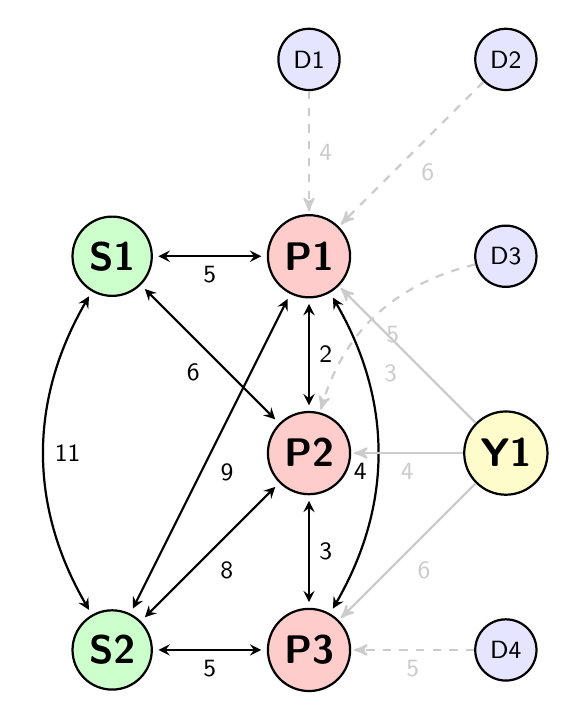
\begin{tikzpicture}[->,>=stealth',shorten >=1pt,auto,node distance=2.5cm,
  thick,yard node/.style={circle,fill=yellow!20,draw,font=\sffamily\Large\bfseries},person node/.style={circle,fill=red!20,draw,font=\sffamily\Large\bfseries}, shelter node/.style={circle,fill=green!20,draw,font=\sffamily\Large\bfseries},
  source node/.style={circle,fill=blue!10, draw,font=\sffamily\small},
  trans/.style={thick,<->,shorten >=2pt,shorten <=2pt,>=stealth}]

  \node[person node]    (1) {P1};
  \node[person node]    (2) [below of=1] {P2};
  \node[person node]    (3) [below of=2] {P3};
  \node[yard node]      (4) [right of=2] {Y1};
  \node[shelter node]   (5) [left of=1] {S1};
  \node[shelter node]   (6) [left of=3] {S2};
  \node[source node]    (7) [above of=1] {D1};
  \node[source node]    (8) [right of=7] {D2};
  \node[source node]    (9) [above of=4] {D3};
  \node[source node]    (10) [right of=3] {D4};
  
  
    

  \path[every node/.style={font=\sffamily\small}, trans]
    (1) edge node []    {2} (2)
        edge node []    {5} (5)
        edge node []    {9} (6)
        edge [bend left] node [below left]    {4} (3)
    (2) edge node []    {3} (3)
        edge node []    {6} (5)
        edge node []    {8} (6)
    (3) edge node []    {5} (6)
    (5) edge [bend right] node []    {11} (6);
    
 \path[every node/.style={font=\sffamily\small},gray!40]
    (4) edge node []    {3} (1)
        edge node []    {4} (2)
        edge node []    {6} (3);
 \path[every node/.style={font=\sffamily\small},gray!40, dashed]
    (7) edge node []    {4} (1)
    (8) edge node []    {6} (1)
    (9) edge [bend right] node     {5} (2)
    (10) edge node []    {5} (3);
\end{tikzpicture}
\caption{Example of a BEP-MA network. Based on [Bish, 2011]}
\label{fig1}
\end{figure}

\subsection{Decision Variables}
$x_{ij}^{mt}$: binary variable that equals $1$ if bus $m$ traverses arc $(i, j)$ on its trip $t$, $0$ otherwise, $\forall \;(i, j) \in A,\; m \in V,\; t = 1, \dots, T$.


$b_{j}^{mt}$: number of evacuees from node $j$ assigned to (or, if $j$ is a shelter, released from) bus $m$ after trip $t$, $\forall \; j \in N, \; m \in V, \; t = 1,\dots, T$.

$z_{j}^{nmrt}$: binary variable that equals $1$ if bus $n$ visits node $j$ on its trip $r$, before bus $m$ visits node $j$ on its trip $t$, $\forall j \in N,\; m \in V, n \in V,\; t = 1, \dots, T,\; r = 1, \dots, T$.

$p_{j}^{nmrt}$: number of evacuees from node $j$ picked up by bus $n$ after its trip $r$, before bus $m$ visits node $j$ after its trip $t$, $\forall j \in N,\; m \in V,\; n \in V,\; t = 1, \dots, T,\; r = 1, \dots, T$.

$T_{evac}$: duration of the evacuation.



\begin{equation}
    \begin{split}
    \text{minimize} \;\;\;T_{evac}\label{eq1}\\
    \end{split}
\end{equation}

subject to

\begin{equation}
    \begin{split}
    T_{evac} \geq \sum_{(i, j)\in A}\sum_{t=1}^{T} \tau_{ij} x_{ij}^{mt}, \;\;\;\forall\; m \in V\\\label{eq2}
    \end{split}
\end{equation}


\begin{equation}
    \begin{split}
    \sum_{i:(i, j)\in A}x_{ij}^{mt} = \sum_{j:(j, k) \in A}x_{jk}^{m(t + 1)},\;\;\; & \forall \; j \in P,\; m \in V, \;\\ & t=1, \dots, T-1\\\label{eq3}
    \end{split} 
\end{equation}

\begin{equation}
    \begin{split}
        \sum_{i:(i,j) \in A}x_{ij}^{mt} \geq \sum_{j;(j, k) \in A}x_{jk}^{m(t + 1)}, \;\;\; & \forall \; j \in S,\; m \in V, \\ & t=1, \dots, T - 1\label{eq4}
    \end{split}
\end{equation}

\begin{equation}
    \begin{split}
        \sum_{(i, j) \in A}x_{ij}^{mt} \leq 1, \;\;\; & \forall \; m \in V, \; t=1, \dots, T\\\label{eq5}
    \end{split}
\end{equation}

\begin{equation}
    \begin{split}
        \sum_{j:(i, j) \in A}x_{ij}^{m1} = 1, \;\;\; & \forall \; i \in Y, \; m \in V_{i}\\\label{eq6}
    \end{split}
\end{equation}

\begin{equation}
    \begin{split}
        x_{ij}^{mt} = 0, \;\;\;\forall\; i \in Y,\; j:(i, j)& \in A,\; m \in V,\\& t=2, \dots, T\\\label{eq7}
    \end{split}
\end{equation}

\begin{equation}
    \begin{split}
        x_{ij}^{mT} = 0, \;\;\;\forall\; j \in P,\; i:(i, j)& \in A,\; m \in V\\\label{eq8}
    \end{split}
\end{equation}

\begin{equation}
    \begin{split}
        b_{j}^{mt} \leq \sum_{i:(i, j) \in A} Qx_{ij}^{mt}, \;\;\; &\forall \; j \in N', \;m \in V, \\& t=1, \dots, T\\\label{eq9}
    \end{split}
\end{equation}

\begin{equation}
    \begin{split}
        0 \leq \sum_{j\in P}\sum_{l=1}^{t}b_{j}^{ml} - \sum_{k\in S}\sum_{l=1}^{t}b_{k}^{ml} \leq Q,\;\;\; &\forall\; m \in V\\
        &t=1, \dots, T\\\label{eq10}
    \end{split}
\end{equation}

\begin{equation}
    \begin{split}
        \sum_{m \in V}\sum_{t=1}^{T}b_{j}^{mt} \leq C_{j}, \;\;\; \forall \; j \in S\\\label{eq11}
    \end{split}
\end{equation}

\begin{equation}
    \begin{split}
        \sum_{m \in V}\sum_{t=1}^{T} b_{j}^{mt} = \sum_{k \in D_{j}}d_{k}, \;\;\; \forall \; j \in P\label{eq12}
    \end{split}
\end{equation}

\begin{equation}
    \begin{split}
        \sum_{j \in P}\sum_{t=1}^{T}b_{j}^{mt} = \sum_{k \in S}\sum_{t=1}^{T}b_{k}^{mt}, \;\;\; \forall \;m \in V\\\label{eq13}
    \end{split}
\end{equation}

\begin{equation}
    \begin{split}
        a^{mt} = \sum_{(i, j)  \in A}\sum_{l=1}^{T}\tau_{ij}x_{ij}^{ml}, \;\;\;& \forall \; m \in V, \;\\&t=1, \dots, T\\\label{eq14}
    \end{split}
\end{equation}

\begin{equation}
    \begin{split}
        e_{j}^{mt} = \sum_{i:(i, j) \in A}x_{ij}^{mt}, \;\;\; &\forall\; j \in N', \; m \in V, \\&t=1, \dots, T\\\label{eq15}
    \end{split}
\end{equation}

\begin{equation}
    \begin{split}
        2 z_{j}^{nmrt} \leq e_{j}^{nr} + e_{j}^{mt}, \;\;\; &\forall \; j \in N, \; \\& n \in V, \; m \in V, \;\\& r=1, \dots, T, \;\\& t=1, \dots, T\\\label{eq16}
    \end{split}
\end{equation}

\begin{equation}
    \begin{split}
        a^{nr} \leq a^{mt} + M (1 - z_{j}^{nmrt}), \;\;\;&\forall \; j \in N, \; \\&n \in V, \; m \in V, \;\\& r=1, \dots, T, \;\\& t=1, \dots, T\\\label{eq17}
    \end{split}
\end{equation}

\begin{equation}
    \begin{split}
        a^{mt} \leq a^{nr} + Mz_{j}^{nmrt} +& M(2 - e_{j}^{nr} - e_{j}^{mt}),\\& \forall \; j \in N, \;  \in V, \; m \in V, \;\\&r=1, \dots, T, \; t=1, \dots, T\\\label{eq18}
    \end{split}
\end{equation}

\begin{equation}
    \begin{split}
        p_{j}^{nmrt} \leq Mz_{j}^{nmrt}, \;\;\;&\forall \; j \in N, \;  \in V, \; m \in V, \;\\&r=1, \dots, T, \; t=1, \dots, T\\ \label{eq19}
    \end{split}
\end{equation}


\begin{equation}
    \begin{split}
        p_{j}^{nmrt} \leq b{j}^{nmrt}, \;\;\;&\forall \; j \in N, \;  \in V, \; m \in V, \;\\&r=1, \dots, T, \; t=1, \dots, T\\ \label{eq20}
    \end{split}
\end{equation}

\begin{equation}
    \begin{split}
        p_{j}^{nmrt} \geq b{j}^{nr} - &M(1 - z_{j}^{nrmt}), \;\;\;\\&\forall \; j \in N, \;  \in V, \; m \in V, \;\\&r=1, \dots, T, \; t=1, \dots, T\\ \label{eq21}
    \end{split}
\end{equation}


\begin{equation}
    \begin{split}
        b_{j}^{mt} \leq \sum_{k \in D_{j}}f(a^{mt};& s_{k}, d_{k}) - \sum_{r=1}^{T}\sum_{n \in V} p_{j}^{nmrt},\;\;\;\\& \forall j\; \in P, \; m \in V, \; t=1, \dots, T\\ \label{eq22}
    \end{split}
\end{equation}



The objective function \eqref{eq1} minimizes the duration of the evacuation. The duration of the evacuation is determined by constraint \eqref{eq2} that, along with \eqref{eq1}, sets the evacuation time equal to the total travel time of the bust with the highest total travel time. Constraint \eqref{eq3} is the flow balance constraint for the pickup nodes and ensures that if a bus visits a pickup node $j$, on trip $t$, it must leave node $j$ on trip $t + 1$. Constraint \eqref{eq4} is the flow balance constraint for shelters, although it allows a bus to stay on the shelter without performing more trips. Constraint \eqref{eq5} ensures a bus traverses at most one arc per trip. Constraint \eqref{eq6} ensures that each bus starts its first trip from its yard. Constraint \eqref{eq7} ensures that the buses do not leave the yard for later trips. Constraint \eqref{eq8} does not allow a bus to end its last trip on a pickup node. Constraint \eqref{eq9} states that a bus only can pickup evacuees from node $j$ if it visits node $j$. Constraint \eqref{eq10} and \eqref{eq11} are the capacity constraints for the buses and shelters respectively. Constraint \eqref{eq12} ensures that all evacuees are picked up, while \eqref{eq13} ensures that all evacuees are delivered to a shelter. Constraints \eqref{eq14} and \eqref{eq15} stands for the variable definitions. Constraints \eqref{eq16} to \eqref{eq18} ensures that the $z_{j}^{nmrt}$ variable satisfy its definition, this is $z_{j}^{nmrt}$ equals $1$ if and only if $e_{j}^{nr}=e_{j}^{mt}=1$ and $a^{nr}\leq a^{mt}$. Constraints \eqref{eq19} to \eqref{eq21} ensures, maintaining model linearity, that $p_{j}^{nmrt} = b_{j}^{nr} z_{j}^{nmrt}$. Finally, constraint \eqref{eq22} ensures that a bus can, at most, pickup the amount of people available at a pickup point at the time when it arrives. The function $f(time;s_{k}, d_{k})$ models, for each source node $k$, the amount of people from that source node that reached the pickup point at a given time. Note that the variables $a^{mt}$ and $e_{j}^{nmrt}$ are not strictly necessary and are introduced only to favor the readability of the model. Also, note that if constraints \eqref{eq14} to \eqref{eq22} are dropped out, the model is equal to the original BEP.

The model was also tested using an alternative objective function, denoted as the cost objective function \eqref{eq23}. This objective was found easier to be solved in \cite{b1} than the min-max objective but doesn't represent the main objective of the problem.
\begin{equation}
    \sum_{(i, j) \in A}\sum_{m \in V}\sum_{t=1}^{T} \tau_{ij}x_{ij}^{mt}
    \label{eq23}
\end{equation}

\subsection{The Arrival Function}

The arrival function contained in \eqref{eq22} seek to model the population behavior after the order of evacuate the area is made. It represents, for a source node $k$, the amount of people that has already arrived to the pickup node at a time $t$. The real process of evacuation is stochastic and $f$ could be modeled with some probability distribution such as the Rayleigh distribution used in \cite{b4} to model the departure probabilities of people on a tsunami evacuation scenario in the Iquique, Chile. However, in order to get a formulation that could be solved using a commercial solver, the arrival function used here is the following:

\begin{equation}
    f(t; s_{k}, d_{k}) = 
    \begin{cases} 
      0 & if \; t\leq s_{k} \\
      ratio * t & if \; s_{k} \leq t \leq \frac{d_{k}}{ratio} + s_{k}\\
      d_{k} & if \; t \geq \frac{d_{k}}{ratio} + s_{k}\\\label{eq24}
   \end{cases}
\end{equation} 

Note that in \eqref{eq24} $t$ stands for time, not for trips. This kind of function also allows to set different ratios for each source node, this could be useful for example if certain areas of the evacuation zone contains a major proportion of elderly people or people with reduced mobility. For experiments, the ratio was obtained by adjusting a linear regression to a Rayleigh distribution, with a average of 20 min, obtaining a ratio of $0.28$.

\section{Computational Results}

This section presents the instances used to test the formulation, along with the computational results obtained. The instances were tested using the original BEP model and the BEP-MA model in order to compare both formulations.

\subsection{Instances}

The formulation was tested in three random instances, constructed on a 5km x 5km frame, and one real-life instance constructed for a flood evacuation scenario in Paipote a zone in Copiap\'o, Chile. Instances are detailed in Table.~\ref{table:inst}. For all instances the bus velocity was considered 60km/h and pedestrian velocity 4,5km/h.
In 2015, the North of Chile suffered a series of floods caused by heavy rainfall that is not frequent in the zone. After this, the government (SERNAGEOMIN) published maps for evacuation in certain zones that are likely to suffer floods in the future. Paipote, with a population of 18,785 persons is one of the most affected areas. Also, the occurrence of floods is likely to be known with some time of anticipation since it flows from the mountain ranges to the coast mainly through riverbeds before reach populated areas. However, a full bus-based evacuation for this area is unlikely because of the great amount of population affected. Because of this, the instance was constructed considering the elder population that live in the area. This data was taken from the 2017 Census. Blocks in the area were clustered using a k-means clustering algorithm (Fig.~\ref{fig2}) to construct 6 pickup points on each cluster centroid, and each block centroid was considered to be a source node. Buses departure from the bus station 'Taxibuses del Sol de Atacama'. The shelters considered are the three nearest public schools that are outside the evacuation zone.  Fig.~\ref{fig3} presents a graphic representation of the instance.
\begin{table}[htbp]

\caption{BEP-MA Instances}
\begin{center}
\begin{tabular}{ cccccc } 
\hline
Instance & Yards & Pickups & Shelters & Buses & Q\\ 
\hline
random1 & 1 & 3 & 2 & 4 & 20\\
random2 & 1 & 4 & 2 & 4  & 20\\
random3 & 1 & 5 & 3 & 6  & 20\\
paipote & 1 & 6 & 3 & 20  & 30\\

\hline
\end{tabular}
\end{center}
\label{table:inst}
\end{table}
\begin{figure}[htbp]
\centerline{\includegraphics{clustered_blocks.png}}
\caption{Clustered blocks, Paipote.}
\label{fig2}
\end{figure}

\begin{figure}[htbp]
\centerline{\includegraphics{paipote_instance.png}}
\caption{Paipote Instace.}
\label{fig3}
\end{figure}

\subsection{Results}
 All instances where tested using the DOcplex API on a Python 3.6 environment with a time limit of 4000 seconds, using a PC with an Intel Celeron N2920 1.86GHz CPU and 8Gb of RAM. All source code is available in \cite{b5}. The compuational results are shown on Table~.\ref{table:res1} for the BEP, and Table~.\ref{table:res2} for the BEP-MA. 
\begin{table}[htbp]

\caption{BEP Results}
\begin{center}
\begin{tabular}{ cccccc } 
\hline
Instance & Objective & Elapsed Time (s) & $T_{evac}$ & Cost\\ 
\hline
random1 & Min-Max & 2.76 & 834.3 & 3250.4\\
random1 & Cost & 0.75 & 970.3 & 2984.4\\
random2 & Min-Max & 4.58 & 839.9 & 3158.7\\
random2 & Cost & 12.92 & 844.1  & 2445.3\\
random3 & Min-Max & 159.4 & 858.3 & 3145.5\\
random3 & Cost & 302.8 & 1198.4  & 2990.7\\
paipote & Min-Max & time limit & 485.2 & 7007.3\\
paipote & Cost & time limit & 652.7 & 6330.0  \\
\hline
\end{tabular}
\end{center}
\label{table:res1}
\end{table}
\begin{table}[htbp]
\caption{BEP-MA Results}
\begin{center}
\begin{tabular}{ cccccc } 
\hline
Instance & Objective & Elapsed Time (s) & $T_{evac}$ & Cost\\ 
\hline
random1 & Min-Max & time limit & 1482.4 & 5780.1\\
random1 & Cost & 1903.9 & 2210.8 & 4791.3\\
random2 & Min-Max & time limit & 2126.0 & 6879.8\\
random2 & Cost & time limit & 2133.1 & 6085.9\\
random3 & Min-Max & time limit & - & - \\
random3 & Cost & time limit & - & - \\
paipote & Min-Max & time limit & - & - \\
paipote & Cost & time limit & - & - \\
\hline
\end{tabular}
\end{center}
\label{table:res2}
\end{table}

The results show that the formulation is very inefficient in terms of computational time. This is expected since the proposed formulation imply the addition of several binary variables that add more complexity to the model increasing the possible combination of variables. Because of this, the solver was capable only to find integer solutions in two of the four instances and found the optimal only in the smaller instance using the cost objective, which is the easier to solve. However, some insights still can be extracted from the results. For the instances that the BEP-MA was capable of finding integer solutions, the optimal value for the total time of evacuation seems to be a lot higher than in the BEP model. This true specially for the first instance, considering that the optimally gap was only 2.7\%. Unfortunately, no solution was found for the BEP-MA for the real case scenario.

\section{Conclusions and Further Work}

This research presented an extension for the BEP proposed in \cite{b1}, by introducing some behavioral characteristics of the population in the model. The results show that both models tested are very inefficient in terms of computational time when solving instances of practical size. This shows that this is a highly combinatorial problem which constitutes an obstacle when trying to apply this models on real life scenarios. However, results suggest that the total evacuation time differs significantly when introducing behavioral characteristics of the population on the model, and therefore is an important aspect to consider at the time of implementation. 

The literature about these kind of model for bus-based evacuation is scarce and must more research on develop heuristic algorithms that can find near-optimal solution in a reasonable time. This is critical thinking on a emergency situation, when the delay in obtaining an evacuation plan could cause an increase in causalities or even deaths. 


\begin{thebibliography}{00}
\bibitem{b1} Bish, D.R., ''Planning for a bus-based evacuation.'' OR Spectrum (2011) 33: 629. https://doi.org/10.1007/s00291-011-0256-1
\bibitem{b2} Dikas, G. Minis, I., ''Solving the bus evacuation problem and its variants.'' Computers \& Operations Research,
vol. 70, pp 75--86, June 2016. https://doi.org/10.1016/j.cor.2015.12.012

\bibitem{b3} Pereira, Victor C. and Bish, Douglas R., ``Scheduling and Routing for a Bus-Based Evacuation with a Constant Evacuee Arrival Rate.'' Transportation Science, vol. 49, no 4, pp 853--867, 2015. https://doi.org/10.1287/trsc.2014.0555
\bibitem{b4} León, Jorge, and Alan March. “An Urban Form Response to Disaster Vulnerability: Improving Tsunami Evacuation in Iquique, Chile.” Environment and Planning B: Planning and Design 43, no. 5 (September 2016): 826–47. doi:10.1177/0265813515597229.
\bibitem{b5} Bus Evacuation Problem with Multiple Arrivals. Available online: https://github.com/scespinoza/bus-evacuation-problem (accesed on July 27 2019).


\end{thebibliography}
\end{document}
